\chapter{Introduction}
Material science applies a broad spectrum of analytical methods for characterisation. For materials where the surface is particularly important, the methods used are the surface sensitive methods. This in itself is a very broad area and includes a large number of complementary methods for investigations of surface composition, structure, reactivity, etc. Here we shall restrict ourselves to the most generally applied methods, such as: The X-ray induced Photoemission Spectroscopy (XPS) also called Electron Spectroscopy for Chemical Analysis (ESCA) and Auger Electron Spectroscopy (AES). These methods can give information on the surface composition and chemistry, and combined with other methods also give information on the lateral and depth composition. Actually any laboratory that is seriously investigating surfaces on the atomic level will have either of these two spectroscopies available. Besides these two rather fundamental methods there are a great number of more special methods which are used in various combinations in order to investigate more complex systems such as the physics of adsorbates and reactions on surfaces. Here we shall go through the most often encountered methods (without making a complete list) which will include Ultraviolet Photoelecton Spectroscopy (UPS), Low Energy Electron Diffraction (LEED), High Resolution Electron Energy Loss Spectroscopy (HREELS), Scanning Tunneling Microscopy etc. 

\section{Area of Application}
Surface scientific methods are used widely both in fundamental and in industrial research laboratories since many technologies require a good understanding of the behaviour of the surfaces. A number of fields can be mentioned such as

\begin{itemize}
\item Catalysis
\item Adhesion
\item Corrosion
\item Tribology
\end{itemize}

Common to all these phenomena is the importance of surface reactivity. Especially in the area of catalysis, surface science has a strong impact for the understanding of what is going on at the atomic level. Surface science is also widely used in other areas like:

\begin{itemize}
\item Metallurgy
\item Biophysics
\item General material synthesis
\item Microelectronics
\end{itemize}

The latter field is probably where most of the analytical methods like Scanning Auger Microscopy (SAM), Auger Electron Spectroscopy (AES), and X-ray Photo-electron Spectroscopy is being brought into use. In general the field of surface science is very cross-disciplinary and is expected to develop continuously with the demand for better materials.

It is the intention here to give a brief introduction to most prominent methods and their applications in material science. For detailed and complete discussion of the various subjects touched upon here we shall refer the reader to references \cite{Zangwill, Somorjai,Hudson,Niemantsverdriet, Ertl,briggs,feldman,woodruff}.

\chapter{Requirements for Surface Analysis}\label{ch:reqs}
In this chapter we shall deal with the two major demands for being able to perform surface analysis. The first requirement may seem at a glance rather trivial but it makes surface science troublesome and expensive. In order to be able to study a surface on the atomic level it is imperative that the cleanliness of the surface can be controlled to a very high degree. Thus all experiments must be performed under \textbf{Ultra High Vacuum}.

\section{Ultra High Vacuum}
Since it is not possible to establish absolute vacuum and as the expenses increases rapidly with the quality of the vacuum it is very important to consider what is really required.

From the kinetic gas theory the velocity distribution is given by a Maxwell-Boltzmann distribution. If we only consider the distribution for molecules with velocity components orthogonal to the surface it can be written as:

\begin{equation}
f(v_x)dv_x = \sqrt{\frac{m}{2\pi kT}}e^{-\frac{mv_x^2}{2kT}}dv_x
\end{equation}

where $k$ is Boltzmann's constant, $m$ is the mass of the gas molecule, and $T$ is the temperature of the gas. The flux $dF(v_x)$ of particles per $v_x$ is proportional to the velocity and the probability distribution.

\begin{equation}
dF(v_x) = v_xf(v_x)dv_x = v_x\sqrt{\frac{m}{2 \pi kT}}e^{-\frac{mv_x^2}{2kT}}dv_x
\end{equation}

Thus the total flux at the surface is easily found by integration over all velocities

\begin{eqnarray}
F &=& \int_{0}^{\infty}f(v_x)v_xdv_x \\
F &=& \int_{0}^{\infty} \sqrt{\frac{m}{2 \pi kT}}e^{-\frac{mv_x^2}{2kT}}v_xdv_x \\
F &=& \sqrt{\frac{kT}{2\pi m}}
\end{eqnarray}

If we want to determine the flux of particles hitting per surface area per time unit this flux has to be weighted by the gas density $\rho$. Assuming an ideal gas $\rho$ can be rewritten as $\frac{P}{kT}$ leading to the final equation

\begin{equation}
F_{tot}(P,T) = \frac{P}{\sqrt{2 \pi mkT}}
\label{eq:total_flux}
\end{equation}

Which implication does this have?

\subsection{Example}
Assume that we have been able to obtain a base pressure of \SI{1e-6}{mbar} oxygen in our vacuum chamber. How long time will it take before every atom on our surface has been hit once on average? We are studying a Cu(100) surface which contains \num{1.5e15} copper atoms per \si{cm^2}. By substitution of the relevant numbers into equation \eqref{eq:total_flux} it is found that the flux at this pressure is \num{2.7e14} \ce{O2} molecules per \si{cm^2} per second. Thus if all the molecules that hit the surface reacts, it will be covered with oxygen within \SI{5}{\second}. As many surface science experiments take hours, it is necessary to reduce the pressure by 4 orders of magnitude leading to Ultra High Vacuum with a base pressure less than \SI{1e-10}{mbar}. How can such low pressure be obtained routinely?


\subsection{Vacuum Equipment}
All experiments must be performed in a container where the vacuum can be established. There are rather strong demands on the materials used. They should have a sufficient low vapour pressure even at temperatures as high as \SI{150}{\degreeCelsius}. This immediately rules out such materials as brass, tin, lead, silver solders containing cadmium, plastic etc. The commonly used materials are stainless steel, glass and ceramics. Usually the vacuum is established by pumping the chamber with a sufficiently good pump and then heat it to at least \SI{150}{\degreeCelsius} for at least 12 hours. This will increase the outgassing from the inner walls considerably so that an adequate base pressure can be obtained when it has cooled down to room temperature.

\subsection{Vacuum Pumps}
The pumps used for this sort of experiments can naturally be divided into two groups: The open types where the gas is removed from the apparatus and the closed types where the gas is captured by implantation, reaction or simply by freezing out in the pump itself.

Usually the apparatus is pumped down from atmospheric pressure by use of open pumping systems as we are dealing with considerable amounts of gas in this situation. A typical combination will consist of a serially connected rough pump ($P_{base} \leq \num{1e-3}$) and a turbopump (see Figure~\ref{fig:turbo_pump}) or an oil diffusion pump (see Figure~\ref{fig:oildiffusion_pump}). Both types of pumps have base pressures around the desired \SI{1e-10}{mbar}.

In the pressure regime below \SI{1e-6}{mbar} the pumping is enforced or done solely by the closed types, like the ion pump (see Figure~\ref{fig:ion_pump}) which removes the gas molecules by a combination of implantation into titanium plates and reaction with freshly exposed titanium.

Another type of a closed pump is the cryo-pump which simply freezes out the gasses by having a very cold region with a large surface area. Both these pumps are very clean and useful. Which pump is used is very much dictated by what sort of experiments that has to be performed as each has its advantages or drawbacks such as:

\begin{itemize} 
\item Ion-pumps \dotfill generates strong magnetic fields
\item Turbo-pumps \dotfill generates vibrations
\item Cryo-pumps \dotfill generates vibrations
\item Oil diffusion-pumps \dotfill requires a constant use of liq. nitrogen.
\end{itemize}

The vacuum chamber must be pumped continuously in order to compensate for outgassing of the walls and any analytical methods installed in the apparatus. If there is a malfunction on the apparatus so it must be vented, the whole procedure of pumping down and baking out must be repeated and a loss of at least one or generally two working days must be faced to re-establish the vacuum.

\begin{figure}[htbp]
\centering
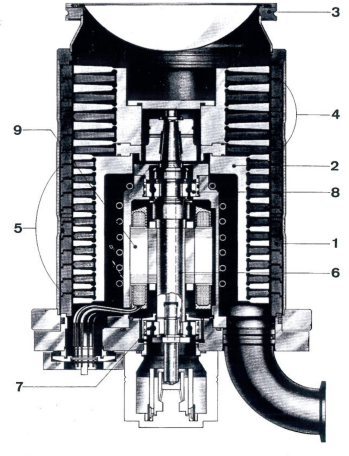
\includegraphics[width=0.5\textwidth]{figures/02_01a}
\caption{Schematic of a turbo pump.}
\label{fig:turbo_pump}
\end{figure}

\begin{figure}[htbp]
\centering
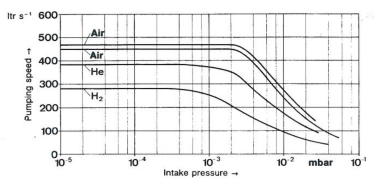
\includegraphics[width=0.6\textwidth]{figures/02_01b}
\caption{Pumping speed as a function of pressure.}
\label{fig:pumping_speed}
\end{figure}

\begin{figure}[htbp]
\centering
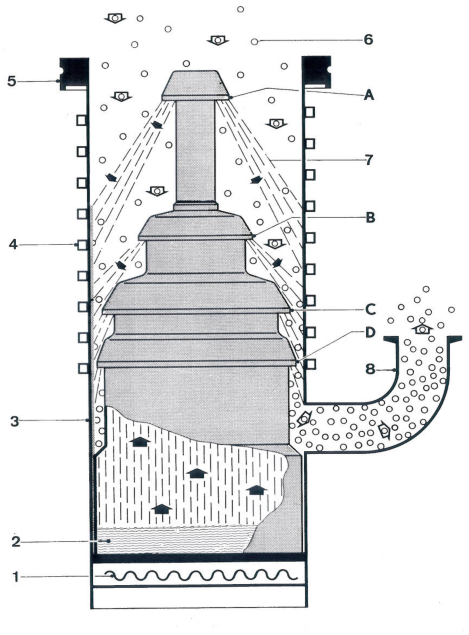
\includegraphics[width=0.5\textwidth]{figures/02_02}
\caption{Schematics of an oil-diffusion pump.}
\label{fig:oildiffusion_pump}
\end{figure}

\begin{figure}[htbp]
\centering
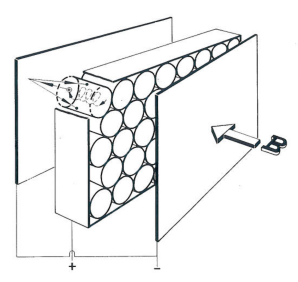
\includegraphics[width=0.4\textwidth]{figures/02_03a}
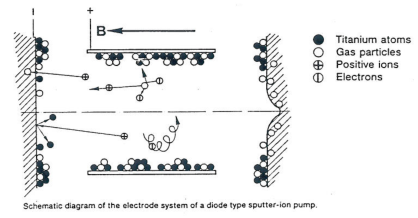
\includegraphics[width=0.5\textwidth]{figures/02_03b}
\caption{Schematics of ion-pumps.}
\label{fig:ion_pump}
\end{figure}

\subsection{Pressure Measurement}
The very low pressure makes the task of measuring the pressures a bit more difficult as all gauges relying on mechanical principles can be ruled out. Usually the pressure is monitored by use of a Bayard-Alpert Ionisation Gauge as shown in Figure~\ref{fig:ion_gauge}.

\begin{figure}[htbp]
\centering
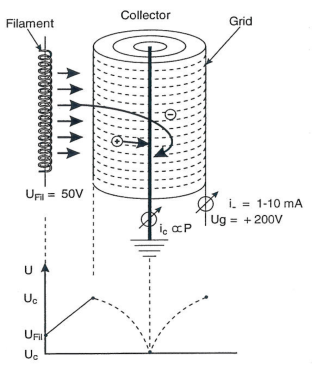
\includegraphics[width=0.5\textwidth]{figures/02_04}
\caption{Schematics of an ionisation-gauge.}
\label{fig:ion_gauge}
\end{figure}

The principle is that electrons are accelerated from a hot filament towards an open structured cage made of a grid. Some electrons will penetrate the cage and be able to ionise gas molecules. In the middle of the cage a thin wire called the collector is mounted which is negatively biased compared to the cage. Positive ions produced by the electron bombardment will be collected by the wire and the current measured will be proportional to the gas density in the cage and thus in the apparatus. Usually such gauges work in the range \SIrange{1e-4}{4e-11}{mbar}. Unfortunately the pressure reading will depend on the gas composition and must therefore be calibrated for the relevant gas.

For more details on Ultra High Vacuum and design of such equipment we shall simply refer to \cite{roth}.

\section{Surface Sensitivity}
The second requirement for doing surface analysis is naturally to have methods that are sensitive to the surface. This in general rules out otherwise useful methods like electron microscopy, X-ray diffraction and M\"{o}ssbauer spectroscopy. The methods inherently applicable for surface investigations are the electron spectroscopies. These methods are relying on the fact that electrons which are passing through a medium will undergo energy losses and thereby have a limited penetration depth. The electron spectroscopies are all performed by excitation of the solid which then will emit electrons with a characteristic energy distribution $N(E)$ that allows for identification of the composition of the solid. The excitation source for generation of these electron energy distributions does not need to be surface sensitive and therefore high energy electrons (AES), X-rays (XPS) or even ions can be used. The important point is that the electrons emitted undergo energy losses on their way out of the solid and therefore electrons coming from inside the solid will be exponentially damped. We shall in later chapters treat the detection, measurements, and interpretation of the emitted electrons and now concentrate on the mechanisms ensuring the surface sensitivity.

\subsection{The Inelastic Mean Free Path}
A useful term for describing the energy loss process is the inelastic mean free path $\lambda (E)$.

\begin{figure}[htbp]
\centering
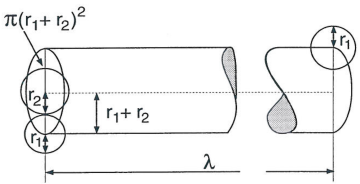
\includegraphics[width=0.5\textwidth]{figures/02_05}
\caption{ }
\label{fig:sphere_model}
\end{figure}

If we consider a hard sphere model, see Figure~\ref{fig:sphere_model}, the mean free path can easily be derived in terms of the cross-section 
\begin{equation}
\sigma = \pi (r_{1}+r_{2})^{2}
\end{equation}
and the density $\rho$. The volume $\lambda \times \sigma$ equals the volume of one molecule which is $\rho^{-1}$ leading to
\begin{equation}
\lambda = (\sigma \rho)^{-1}
\end{equation}

For a frozen ideal gas this would give
\begin{equation}
\lambda = \frac{kT}{\sigma P}
\end{equation}
Taking into account the relative motion of the molecules the result is
\begin{equation}
\lambda = \frac{kT}{\sqrt{2} \sigma P}
\end{equation}

Similar considerations can be made for electrons moving in a solid matter except that the cross-section is much more complex and dependent on the underlying mechanism. Below we shall describe the different mechanisms and their importance.

The important result of these mechanisms are summarised in Figure~\ref{fig:mean_free_path} where the inelastic mean free path for electrons is plotted against the electron energy in a number of different materials.

\begin{figure}[htbp]
\centering
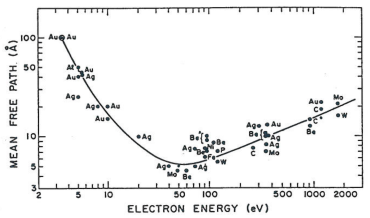
\includegraphics[width=0.7\textwidth]{figures/02_06}
\caption{The inelastic mean free path versus kinetic energy for a number of elements.}
\label{fig:mean_free_path}
\end{figure}

Notice that the mean free path is only a few atomic layers if we design our experiments so that the electrons have energies in the interval \SIrange{50}{1000}{\electronvolt}.

\subsection{The Energy Loss Mechanisms in Solids}
There are a number of different energy loss mechanisms that are responsible for the behaviour of the inelastic mean free path observed in Figure ~\ref{fig:mean_free_path}.

We shall here consider the various mechanisms in the order of decreasing importance. Excitations of collective charge density waves also called plasmons is one of the most important mechanisms for energy loss of electrons in a solid medium with valence electrons. Consider a free electron metal like aluminium. The three valence electrons are highly delocalised and the system can be described relatively well by a jellium model where the electrons are smeared out on a background of positive charge. If we introduce a small perturbation of the charge densities of the electrons with respect to the positive background as shown in Figure~\ref{fig:plasmon_derive} we can estimate the forces introduced on the volume element $dV$.

\begin{figure}[htbp]
\centering
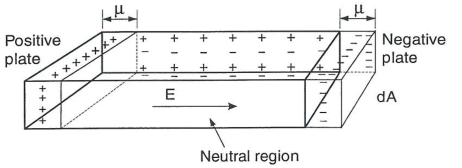
\includegraphics[width=0.5\textwidth]{figures/02_07}
\caption{A sketch of the simple system used to derive the energy losses due to plasmons.}
\label{fig:plasmon_derive}
\end{figure}
 
The volume element will have a charge of electrons which is

\begin{equation}
dq = n\mu edA
\end{equation}

where $n$ is the electron density, $\mu$ is the displacement, $e$ is the electronic charge, and $dA$ is the area element. We can consider the two end plates of the box as a capacitor whereby we have the electric field $E$

\begin{equation}
E = \frac{dq}{dA\varepsilon_{0}}=\frac{ne\mu}{\varepsilon_{0}}
\end{equation}


By having the electric field we can apply Newton's 2nd law
\begin{equation}
m\frac{d^{2}\mu}{dt^2}= F_{electron}=-eE=-\frac{ne^2\mu}{\varepsilon_0}
\end{equation}

This is a simple 2nd order differential equation describing a harmonic oscillator with the frequency $\omega_{p}$

\begin{equation}
\omega_p = \sqrt{\frac{ne^2}{\varepsilon_0 m}}
\end{equation}

For typical free electron metals like Mg and Al the models predict plasmon energy losses of \SIlist{10.9;15.8}{\electronvolt} respectively which is in good agreement with the observed values of \SIlist{10.6;15.3}{\electronvolt}.

This simple model does not work as well for metals where the valence electrons are more localised as is the case for the d-electrons in the transition metals.

By simple considerations of the electric field and its boundary conditions at the surface, it can be shown that a special type of plasmons can be excited in this region namely the surface plasmons. These plasmons will have a frequency which is $\omega_{s} = \frac{\omega_{p}}{\sqrt{2}}$.

The effect of the plasmon energy losses is easily observed by bombardment of a clean aluminium surface with electrons with increasing energy $E_{p}$. By analysing the electrons reflected from this surface, as illustrated in Figure~\ref{fig:plasmon_loss}, the $N(E)$ distribution shown in Figure~\ref{fig:plasmon_spectra} is observed.
\begin{figure}[htbp]
\centering
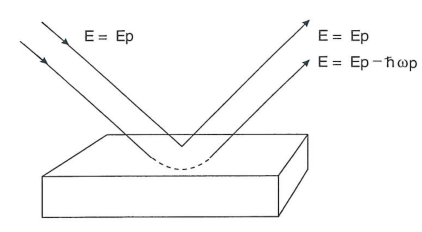
\includegraphics[width=0.5\textwidth]{figures/02_08}
\caption{ }
\label{fig:plasmon_loss}
\end{figure}

\begin{figure}[htbp]
\centering
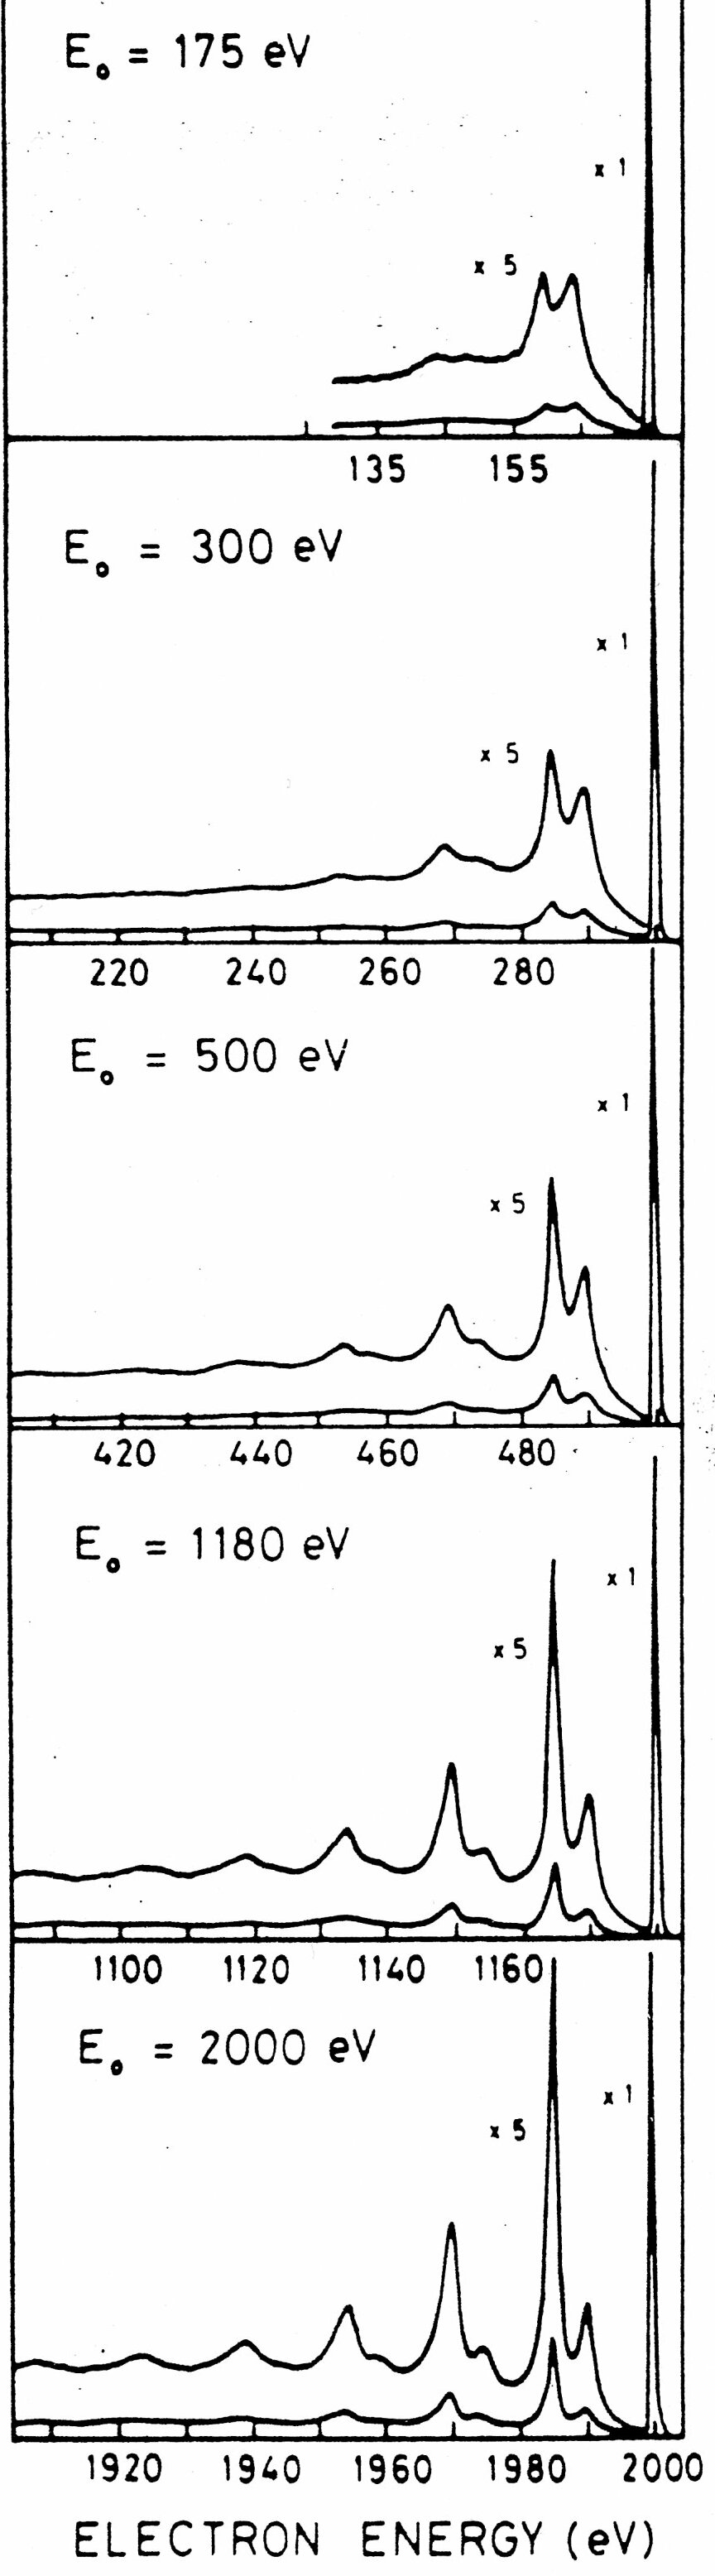
\includegraphics[width=0.2\textwidth]{figures/02_09}
\caption{The energy loss spectra of aluminium for various primary energies.}
\label{fig:plasmon_spectra}
\end{figure}

The feature at the primary energy $E_{p}$ is due to electrons which are elastically reflected. The features observed towards lower energies are the electrons which have undergone one or more energy losses. The bulk and the surface plasmons are easily seen and notice how the number of energy losses increases with increasing primary energy. Thus electrons emitted from within the aluminium will show similar energy loss spectra, although the surface contribution will only be half compared to the spectra shown in Figure~\ref{fig:plasmon_spectra} as they only have to pass the surface once.

The next mechanism for energy loss is ionisation of the atoms in the solid. In the scattering process the electron loses enough energy so that a bound electron can be lifted above the Fermi level of the solid and here occupy an empty state. The process is illustrated in Figure~\ref{fig:discrete_losses} where high energy electrons are transmitted through a \SI{500}{\angstrom} thin film of \ce{NiAl}.

\begin{figure}[htbp]
\centering
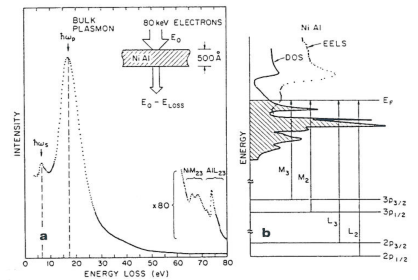
\includegraphics[width=0.5\textwidth]{figures/02_10}
\caption{Discrete energy losses observed by transmission of \SI{80}{k\electronvolt} electrons through a \ce{NiAl} alloy.}
\label{fig:discrete_losses}
\end{figure}

Again we clearly identify the plasmon losses, but if we look carefully towards higher energy losses the energy loss by excitation of the 2p electrons of aluminium and the 3p electrons of nickel can be observed. The energy losses observed fit very well with the excitation of the p electrons to just above the Fermi level as indicated in Figure~\ref{fig:discrete_losses}. Larger energy losses are also possible, but will not lead to such distinct structure in the energy loss spectrum. The cross section for this type of excitation can be approximated by

\begin{equation}
\sigma(E) \approx N_x\frac{ln(\frac{E}{I_x})}{E}
\end{equation}
where $E$ is the energy of the electron, $N_x$ is the number of electrons in subshell $x$, and $I_x$ is the energy required for ionisation of this level. It is easily shown that this cross section has a maximum for electrons with an energy roughly three times the ionisation energy. The cross section plotted against $\frac{E}{I}$ is shown in Figure~\ref{fig:discrete_losses_crosssection}. The same type of cross section behaviour also applies to excitations of plasmons.

\begin{figure}[htbp]
\centering
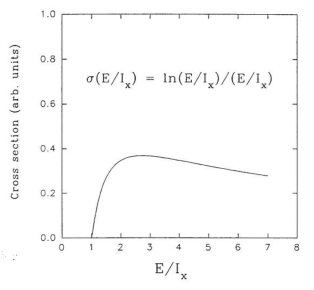
\includegraphics[width=0.5\textwidth]{figures/02_11}
\caption{The cross-section for discrete energy loss as a function of energy.}
\label{fig:discrete_losses_crosssection}
\end{figure}

Although the primary energy used in Figure~\ref{fig:discrete_losses} is atypical for the surface science experiments the relative importance of the two mechanisms is clearly seen. In general the ionisation process will always be present and as we shall see in a later chapter this mechanism actually forms the basis for the Auger Electron Spectroscopy which is nothing else but the relaxation process following such excitation processes.

The next process is weak and contrary to the two previous energy loss mechanisms only involves losses of small energy quanta. Excitations of excitons or electron-hole pairs are usually very small \SIrange{0}{2}{\electronvolt} and involve excitations of the valence electrons into the empty conduction band. Thus for a metal this will lead to a rather smooth energy loss feature proportional to the joint density of states between the valence band and the conduction band (see Figure~\ref{fig:schem_exitons}).

\begin{figure}[htbp]
\centering
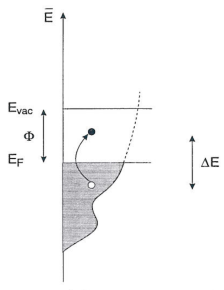
\includegraphics[width=0.3\textwidth]{figures/02_12}
\caption{Schematics showing excitations of excitons (electron-hole pairs).}
\label{fig:schem_exitons}
\end{figure}

The phenomenon may also lead to distinct structures in for example semi-conductors where there are distinct bands and a band gap. The same mechanism leads to the so-called Doniach-Sunjic line shapes in the core level spectra observed with XPS as we shall see in Chapter \ref{ch:xps}.
%REMEMBER TO CHANGE THIS REFERENCE TO A LABEL!!!

Another very weak energy loss process is the excitation of phonons or lattice vibrations. The energy quanta involved here are continuous as the phonons form dispersion bands usually below \SI{50}{m\electronvolt}. Higher and discrete energy losses can be observed for adsorbed molecules on surfaces depending on the adsorption site and the metal, an adsorbed CO molecule will have an energy loss of ~\SI{260}{m\electronvolt} for instance. This energy loss mechanism is very important for investigations of adsorbed molecules and the method is called High Resolution Electron Energy Loss Spectroscopy (HREELS). An example is shown in Figure~\ref{fig:formate_spectrum} where a HREELS spectra was measured of formate adsorbed on Cu(100).

The electron energy was only \SI{4.2}{\electronvolt} and the various energy losses are easily identified and an isotope effect can be observed on the C-H stretch vibration when hydrogen is replaced by deuterium. This phonon loss mechanism is not very important in AES and XPS, but it is the mechanism responsible for the well known phenomenon resistivity.

For completeness we shall also mention that electrons which are accelerated will emit radiation \cite{Feynman} and therefore also undergo continuous energy losses when scattered in the solid. It is not identified in the energy loss spectra as it is such a weak effect, but if we consider the radiation from a solid bombarded with high energy electrons it can be observed as indicated in Figure 4.5.
%REMEMBER TO CHANGE THIS REFERENCE TO A LABEL!!!

\begin{figure}[htbp]
\centering
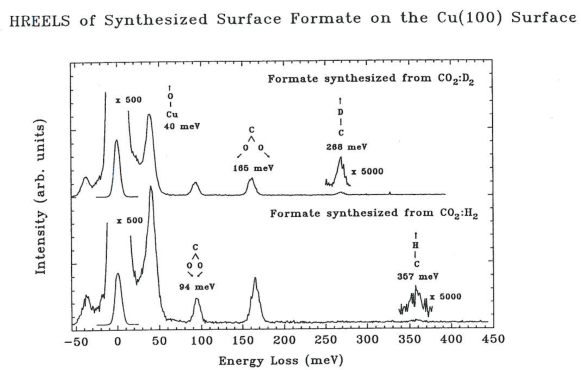
\includegraphics[width=0.5\textwidth]{figures/02_13}
\caption{Energy loss spectrum of formate adsorbed on Cu(100). The primary energy of the electrons was \SI{4.2}{\electronvolt} and the resolution was \SI{8}{m\electronvolt}.}
\label{fig:formate_spectrum}
\end{figure}

\section{Problems}
\begin{enumerate}
\item Another type of pump, called a titanium sublimation pump, can be constructed. This pump relies on the high reactivity of titanium. By heating a filament made of a \ce{TiMo} alloy, Ti will be sublimated out on the surrounding walls (which may or may not be cooled). Assume that a cylinder with a radius of \SI{.1}{m} and height of \SI{.1}{m} is covered with freshly evaporated titanium. The base pressure in the chamber is \SI{1e-9}{mbar}.\\

Estimate the pumping speed of this surface. (Hint: Choose a gas present in the chamber e.g. \ce{N2})\\

Are there gases which cannot be pumped by this pump?\\

In the following we shall assume that the rest gas consist of nitrogen and that the pressure is kept constant. How long time will it take before the pumping speed of the evaporated titanium is reduced to \SI{10}{\percent} of its initial speed?\\

\item Determine the mean free path of a nitrogen molecule at \SI{1}{mbar} and at \SI{1e-6}{mbar}. At what pressure is the mean free path smaller than the dimension of an apparatus?

\item Determine the density of valence electrons in Mg and Al. What is the energy of a surface plasmon on metallic Ca?
\end{enumerate}

\chapter{Energy Analysis}\label{ch:ea}
In the following we shall be able to measure the energy distribution of electrons emitted from a surface in the energy range from \SIrange{10}{2000}{\electronvolt} with a reasonable resolution. The energy analysis is done by electrostatic energy analysers where electrons are selected by a combination of geometry and potentials. Here we shall only consider the two most popular energy analysers, the Concentric Mirror Analyser (CMA) and the Hemi-Sperical Energy Analyser (HSA).

\section{The Concentric Mirror Analyser}
The CMA is used mainly for AES where less resolution is necessary, typically \SIrange{1}{10}{\electronvolt}. The analyser consists of two concentric cylinders as shown in Figure~\ref{fig:schematics_cma}. The inner cylinder is grounded whilst the outer cylinder is ramped at a negative potential. An electron gun is mounted inside the inner cylinder. In the front there is a defining aperture and the electrons having the appropriate energy defined by the outer cylinder will pass the exit slit and be detected by an electron multiplier. Electrons which do not have the energy defined by the potential difference between the inner and outer cylinder will not be able to pass and are therefore not detected. It can be shown that this set-up is imaging the sample onto the exit slit in front of the channeltron if the geometry is designed correctly. That geometry is obtained if the take-off angle through the entrance slit is \ang{42.18}. Since the analyser has a transmission efficiency of roughly \SI{10}{\percent} it is a relatively efficient analyser. The only major drawbacks on a CMA is that the sample has to be located close to the analyser and the limited resolution. If for instance \SI{1000}{\electronvolt} electrons are to be measured with a typical CMA which has a resolution of \SI{0.6}{\percent} the feature measured at this energy will be \SI{6}{\electronvolt} broad. This is satisfactory for analysis of Auger electrons but certainly not for XPS studies. Higher resolution can be obtained by having two CMA's in series. This is called a Double Pass CMA, but better solutions have been developed.

\begin{figure}[htbp]
\centering
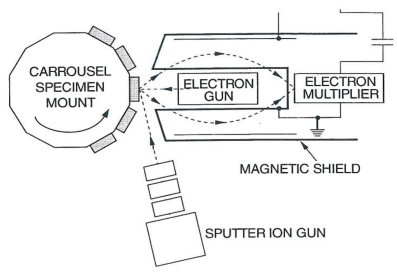
\includegraphics[width=0.5\textwidth]{figures/03_01}
\caption{Schematics of a CMA.}
\label{fig:schematics_cma}
\end{figure}

\section{The Hemi-Spherical Analyser}
For XPS there is a demand for an energy resolution better than \SI{1.0}{\electronvolt} or preferably \SI{0.5}{\electronvolt} over a broad energy range, \SIrange{0}{1500}{\electronvolt}. This is obtainable by applying a different set-up, the so called HSA as shown in Figure~\ref{fig:schematics_hsa}. This analyser consists of two concentric hemi-spheres with an entrance slit and a detector. Usually a lens system will guide the electrons from the sample to the entrance slit by imaging the sample onto the entrance slit. At the entrance slit there is mounted a retarding grid which only allows electrons with a certain energy to pass. The same grid also determines the potential of the central path between the two hemi-spheres. The potential difference between the two spheres determines a pass energy at which electrons will be able to travel through the analyser and be detected at the exit slit where an electron channeltron is mounted. Thus the geometry images the entrance slit on the exit slit.

\begin{figure}[htbp]
\centering
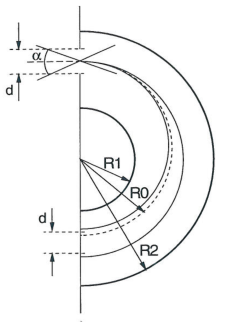
\includegraphics[width=0.3\textwidth]{figures/03_02}
\caption{Schematics of a HSA.}
\label{fig:schematics_hsa}
\end{figure}

Again the resolution is a constant percentage of the pass energy (roughly SI{1}{\percent}) and it is therefore desirable to only use low pass energies, typically \SIrange{5}{100}{\electronvolt}. On the other hand everything has its price. A high resolution means low signal and thus poor signal to noise ratio. It is therefore always important to realise what level of resolution is necessary.

The electrons that have an energy that allows them to pass through the exit slit are detected by an electron multiplier. This is a ceramic tube covered on the inside with a material from which electrons are easily knocked out (see Figure~\ref{fig:electron_multiplier}).

\begin{figure}[htbp]
\centering
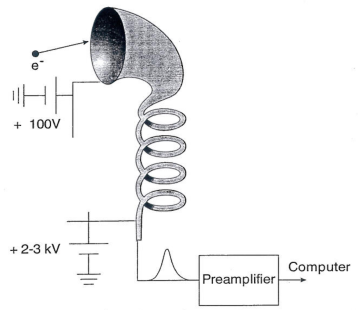
\includegraphics[width=0.5\textwidth]{figures/03_03}
\caption{Schematics showing an electron multiplier.}
\label{fig:electron_multiplier}
\end{figure}

The front of the multiplier is typically at  \SIrange{100}{200}{V} while the end is at \SIrange{2}{3}{kV}. Thus electrons are accelerated into the channeltron where they eventually will hit the wall and knock out other electrons which again are accelerated. In this manner a cascade is formed and one electron may become \numrange[range-phrase = --]{10^6}{10^7} in the other end. This is a fairly big pulse which can easily be detected by some preamplifier and converted into a signal that the computer can handle.

The transmission efficiency for both types of analysers depends on the energy of the electrons. Thus when quantitative or comparative studies are undertaken it is important to take into account the transmission function. We shall come back to this under the discussion of quantitative studies of surface composition.

\subsection{Example}
Determine what the potential should be on the retarding grid and the two hemi-spheres if we want to detect \SI{1000}{\electronvolt} electrons with a resolution of \SI{0.2}{\electronvolt} with an HSA which has $R_{1}=\SI{0.10}{m}$ and $R_{2}=\SI{0.15}{m}$.

A resolution of \SI{0.2}{\electronvolt} means that the pass energy should be \SI{20}{\electronvolt} and the retard potential must then be $\SI{-1000}{V}+\SI{20}{V}=\SI{-980}{V}$. This is also the potential right in the middle of the two hemi-spheres $V_{0}$. The electric field between the two hemi-spheres can be found by use of Gauss law

\begin{equation}
\int \vec{E}(r)d\vec{s}=\frac{q}{\epsilon_0}
\end{equation}

by using that

\begin{equation}
\vec{E}(r)=-\vec{\nabla}V(r)
\end{equation}

we can by integration using the appropriate boundary conditions get

\begin{equation}
V(r)=V_0 + \frac{q}{2\pi \epsilon_0}\left(\frac{1}{r}-\frac{1}{R_0}\right)
\end{equation}

where $R_0=\left(R_1+R_2\right)/2$. The force necessary for the orbit motion is supplied by the electric field

\begin{equation}
\vec{F_{c}}=\vec{F_{E}}
\end{equation}

leading to

\begin{equation}
\vec{E}(R_0)=\frac{mv^{2}}{R_0e}=\frac{2E'_{kin}}{R_0e}
\end{equation}

where

\begin{equation}
E'_{kin}=E_{kin}-V(R_0)e
\end{equation}

is the kinetic energy of the electron after it has passed the retarding grid. By elimination of $q$ it is easily found that the potential between the spheres can be described by

\begin{equation}
V(r)=\frac{2E'_{kin}}{e}\left(\frac{R_0}{r}-1\right)+V_0
\end{equation}

In this manner the potential of the inner and outer hemi-spheres is found to be \SIlist{-970;-988}{V} and respectively. Notice that the resolution in this set-up will be constant as we are using constant pass energy.
